\chapter{静磁现象}



\begin{definition}[磁性]
    外磁场改变时,系统能量随之改变的性质。
\end{definition}


%——————————————————————————————————%
\section{磁矩}
\begin{definition}[磁荷]
    假设的仅带有北极或南极的单一磁极的基本粒子。
    \[ F = \frac{1}{4\pi\mu_0} \frac{m_1m_2}{r^2_{12}} \]
    其中$\mu_0=4\pi \times 10^{-7} H/m$, $m$单位为$Wb$。
\end{definition}

\begin{proposition}[磁力矩]
    一个大小为$m$的磁极放入大小为$H$的场所受的力$F=mH$。
    磁极成对出现致使匀强场中合力为零,力矩为$L=-mlH\sin{\theta}$。
    非匀强场中合力为$F=mH_1-mH_2=m(\Delta H)$。
    当$l\to0$时,$\Delta H \approx l\frac{dH}{dx}$。
\end{proposition}

\begin{definition}[磁矩]
    磁矩:
    \[M=ml\]
    其转矩与势能:
    \begin{align*}
        \vec{L} &= \vec{M} \times \vec{H} \\
        U &= -\vec{M} \cdot \vec{H}
    \end{align*}
\end{definition}



%——————————————————————————————————%
\section{磁性材料和磁化强度}

% \begin{definition}[磁性材料]
%     受磁场作用时显示出某种磁性的材料。
% \end{definition}
\begin{definition}[磁化强度]
    单位体积内,材料中磁矩的总和。
    \[\vec{I}=\frac{1}{v}\sum^{n}_{i=1}\vec{M_i}\]
\end{definition}
\begin{remark}
    $M$为磁化强度,$I=\mu_0M$为磁极化强度。$I$的单位为$Wb\times m/m^3=Wb/m^2=T$
\end{remark}


对磁化强度的理解:
\begin{enumerate}
    \item 磁矩观点;
    \item 磁极(荷)观点:若所有磁矩平行排列,且大小相等。
    \[I=NM=Nml=\rho l\]
    $N$为单位体积内的磁矩数,$\rho$为磁荷密度。
    $I$可以解释为$+\rho$和$-\rho$相对位移$l$距离,在表面出现未被补偿的磁荷,
    表面密度$\omega=\rho l$,故$I=\omega$
    
    \item 分子环流观点:相邻电流方向相反抵消,只有侧面电流环。
    每单位长度有$n$个电流环,每个电流环的面积$S$。
    \[I=NM=\frac{n}{S}(\mu_0iS=\mu_o(ni)=\mu_0H'\]
    $H'$为内部的分子环流磁场。
\end{enumerate}

\begin{definition}[磁通密度]
    材料的磁化强度与真空磁化强度之和。
    \[B=I+\mu_oH=\mu_0(H'+H)\]
\end{definition}

\begin{definition}[磁通量]
    通过某给定曲面的磁场(亦称为磁通量密度)的大小的度量。
    \[\Phi = BS\]
    \[\Phi = \int_s\vec{B}\,d\vec{S}\]
\end{definition}

\begin{definition}[磁导率]
    某种材料对一个外加磁场线性反应的磁化程度。\\
    电磁感应:
    \[ V = -\frac{d\Phi}{dt} \]
    空心线圈:
    \[ V_0 = -N \frac{d(BS)}{dt} = -NS\mu_0 \frac{dH}{dt} \]
    有磁性材料:
    \[ V_m = -NS\frac{dI}{dt} - NS\mu_0 \frac{dH}{dt} \]
\end{definition}
\begin{remark}
    若$I = \chi H$(通常不成立),$\chi$磁导率;
    $B = (\chi + \mu_0)H$,$\mu$磁导率。
\end{remark}

工程上,用相对$\mu_0$的无量纲值。
\begin{align*}
    \mu_r &= \frac{\mu}{\mu_0} \\
    \chi_r &= \frac{\chi}{\mu_0} \\
    B &= \mu_0 \mu_r H
\end{align*}
\[ V_m = -NS\frac{dB}{dt} - NS\mu_0\mu_r \frac{dH}{dt}
    = \mu H
\]

空心线圈插入磁性材料,会使电磁感应效应提升$\mu_r$倍。



%——————————————————————————————————%
\section{铁磁材料的磁化强度和退磁场}
\begin{enumerate}
    \item 初始磁化曲线:
    \begin{center}
        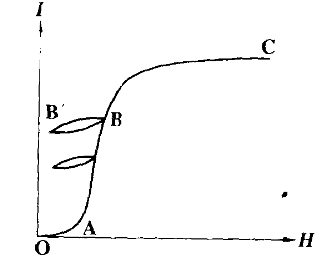
\includegraphics[scale=0.8]{images/1_2.png}
        \captionof{figure}{初始磁化曲线}
    \end{center}
    \begin{enumerate}
        \item 退磁状态(起始)$H=0$,$I=0$。
        $I$随着$H$沿OABC非线性变化。
        \item OA段:$I$和$H$几乎线性变化且可逆。
        \item AB段:$I$增加快,发生不可逆磁化。($H$减小,并不会沿BA返回)
        \item BC段:趋近饱和
        \item C点:饱和点,$I$不再随$H$增大而增大。
            $I_s$为饱和磁化强度。
    \end{enumerate}
    \item 磁滞回线:
    从$+H_m$(饱和)减小到零,反向到$-H_m$,然后回到$+H_m$,形成一个磁化闭环时,
    $I \sim H$的变化曲线。
    \begin{center}
        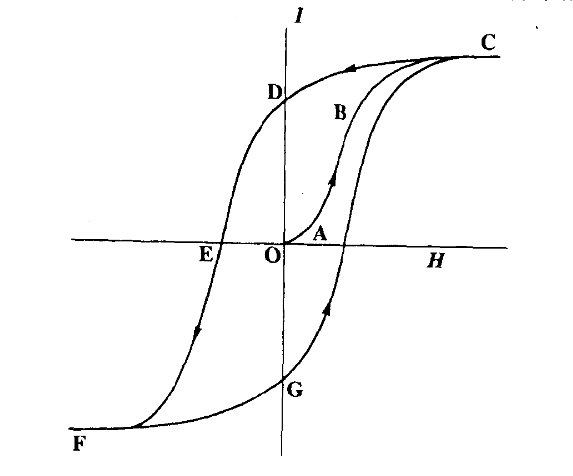
\includegraphics[scale=0.5]{images/1_1.png}
        \captionof{figure}{磁滞回线}
    \end{center}
    \begin{enumerate}
        \item CD段:$H$减小,但不沿着CBAO回去,在$H=0$具有非零的$I_r$,即剩余磁化强度。
        \item 反向加场:$I$减小到零,对应场记做$-H_c$,即矫顽场。
        \item EF段:负向趋近饱和$-I_s$(F点)
        \item FGC段:回到正向饱和。
    \end{enumerate}

    \item 退磁场:有限大小磁体在其两端出现的自由磁极产生与$I$方向相反的内部磁场。
    \[ H_d = N\frac{I}{\mu_0} \]
    $N$为退磁因子,只与样品形状有关。

    退磁因子本质与磁偶相互作用有关。
    \begin{proposition}
        退磁因子对任意椭球,内部$I$处处相等。
        \begin{enumerate}
            \item 球体:$N_x=N_y=N_z=\frac{1}{3}$
            \item 细长圆柱:$N_z \approx 0 \\ N_x=N_y=\frac{1}{2}$
            \item 薄膜:$N_z = 1 \\ N_x=N_y=0$
        \end{enumerate}
    \end{proposition}

    \item 退磁校正:校正回线不依赖磁体形状,只反映材料磁特性。
    \begin{center}
        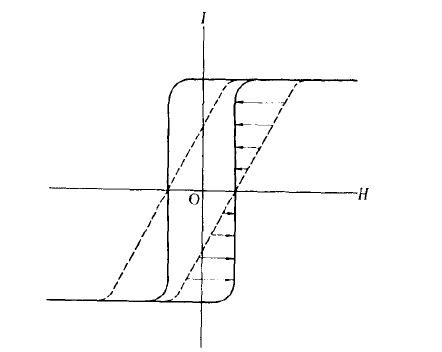
\includegraphics[scale=0.7]{images/1_3.png}
        \captionof{figure}{校正回线}
    \end{center}

    \item 磁体空腔内的有效场:$H_{in} = N \frac{I}{\mu_0}$,
    $N$为形状同空腔的磁体的退磁因子。
    \begin{center}
        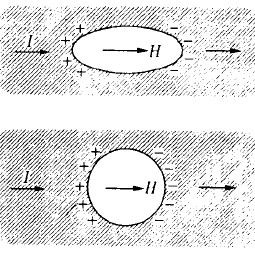
\includegraphics[scale=0.8]{images/1_4.png}
        \captionof{figure}{磁体空腔内的有效场}
    \end{center}
\end{enumerate}



%——————————————————————————————————%
\section{磁路}
高磁导率材料,倾向于把磁力线封闭与于内部。

类比于电路:
\[I = \iint \vec{j} \,d\vec{S}\]
\begin{align*}
    \epsilon 
    &= \oint_L Edl = \oint_L \frac{\vec{I}}{\sigma}dl\\
    &= \sum_i \frac{j_i s_i}{\sigma_i s_i} l_i
        = I \sum_i \frac{l_i}{\sigma_i s_i} \\
    &= I(R_1 + R_2 + ...) = IR_{tot}
\end{align*}

\newpage

磁路:
\[\Phi = \iint \vec{B} \,d\vec{S}\]
\begin{align*}
    NI_0 
    &= \oint_L Hdl = \oint_L \frac{\vec{B}}{\mu}dl\\
    &= \sum_i \frac{B_i s_i}{\mu_i s_i} l_i
        = I \sum_i \frac{l_i}{\mu_i s_i} \\
    &= \Phi(R_{m_1} + R_{m_2} + ...) = IR_{m_{tot}}
\end{align*}

利用永磁体提供磁动势:
\begin{center}
        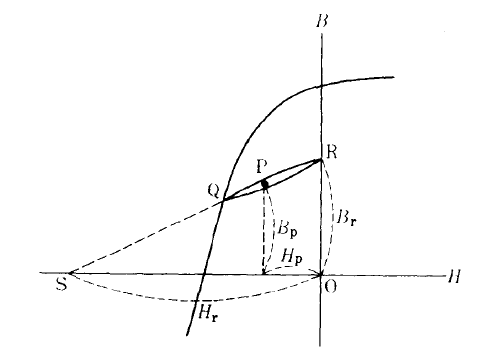
\includegraphics[scale=0.7]{images/1_5.png}
        \captionof{figure}{永磁体的退磁曲线}
\end{center}

孤立永磁体状态于Q,放入磁路后其$H_d$减小至P。视PQR为可逆小回线有可逆磁导率$\mu_{rev}$。
永磁体于R时状态等效为$B_r=\mu_{rev}H_r$的软磁,其磁动势:
\[ \epsilon_m = -H_rl = \frac{B_rl}{\mu_{rev}} \]



%——————————————————————————————————%
\section{静磁能}
铁磁体能量来自原子尺度的静磁效应,由自能与外场能组成。
\begin{definition}[自能]
    磁矩$\vec{M}$在$\vec{H}$中能$-\vec{M} \cdot \vec{H}$

    视铁磁体含有多个$\vec{M_i}$,则
    \[U_\text{自}=-\frac{1}{2}\sum_i\vec{\mu_i}\vec{H_i}\]

    \begin{enumerate}
        \item 积分形式I:
        \[U_\text{自}=-\frac{1}{2}\int_V\vec{I} \cdot\vec{H_d} d^3\vec{r} 
        {-\frac{1}{2}\int_V\vec{I} \cdot\vec{H_d} d^3\vec{r}}_\text{磁体内}\]
        \item 积分形式II:
        \[U = -\frac{1}{2}\int\mu_0 H_d^2 d^3\vec{r}
        {=-\frac{1}{2}\int\mu_0 H_d^2 d^3\vec{r}}_\text{全空间}\]
    \end{enumerate}
\end{definition}

例:孤立磁体的 
\[\frac{1}{2} \int \vec{B} \cdot \vec{H} \cdot d^3\vec{r} = 0\]

由:
\begin{align*}
    \vec{B} \cdot \vec{H} 
    &= \vec{H} \cdot (\vec{\nabla} \times \vec{A})\\
    &= \vec{\nabla} \cdot (\vec{A} \cdot \vec{H})
        + \vec{A} \cdot (\vec{\nabla} \cdot \vec{H})
\end{align*}

有:
\begin{align*}
    \frac{1}{2}\iiint\vec{B} \cdot \vec{H} d^3\vec{r}
    &=  \frac{1}{2}\iiint\vec{\nabla} \cdot (\vec{A} \cdot \vec{H})
        d^3\vec{r}\\
    &=  \frac{1}{2}\oint \vec{A} \cdot \vec{H} dS
        {\frac{1}{2}\oint \vec{A} \cdot \vec{H} dS}_{r\to \infty}\\
    &= 0
\end{align*}

磁化过程中外场做功:
\[ \vec{H} = \vec{H_{ex}} + \vec{H_d} \]
\[ d\vec{B} = d\mu_0\vec{H_{ex}} + d\mu_0\vec{H_d} + dI \]

系统:
\begin{align*}
    \delta w 
    &= \int_\text{全} \vec{H} \cdot d\vec{B} d^3 \vec{r}\\
    &= \int_\text{全} (H_{ex}+H_d)(\delta \mu_0 \vec{H_{ex}} 
        + \delta \mu_0 \vec{H_{d}} + \delta I) d^3 \vec{r}\\
    &= \underbrace{\int H_{ex} \delta(\mu_0 \vec{H_{ex}}) d^3\vec{r}}
        _\text{磁场对真空做功}\\
    &+ \underbrace{\int\mu_0 (\vec{H_{ex}}\delta\vec{H_d} + 
       \vec{H_d} \delta \vec{H_{ex}}) d^3 \vec{r}}
        _{\int\mu_0\delta(H_{ex} \cdot H_d) d^3 r = 0}\\
    &+ \underbrace{\int H_d\delta(\mu_0H_d)d^3\vec{H}}
        _{\delta U_\text{自}}\\
    &+ \underbrace{ \int H_d \delta I d^3\vec{H}}
        _{-\delta U_\text{自}}\\
    &+ \underbrace{\int H_{ex}\delta I d^3\vec{H}}
        _\text{外场对磁体做功}
\end{align*}

外场做功:
\[ W_\text{外} = \int^{I_2}_{I_1}H_{ex}dI\]



%——————————————————————————————————%
\section{软磁和硬磁}
在初始磁化曲线中,外场将磁体从初始化到饱和所做功的面积为:
\[ \int_o^{I_s} H_{ex}\,dI \]
\begin{center}
    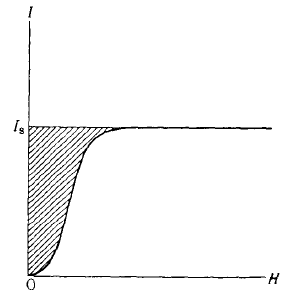
\includegraphics[scale=0.7]{images/1_6.png}
    \captionof{figure}{初始磁化曲线}
\end{center}

在磁滞回线中,磁滞损耗为:$\oint \vec{H}d\vec{I}$

对于软磁:$\chi=I_S/H_S$,$\mu=B/H$

储能为:
\[ V\int_0^H \vec{H} \cdot x \,dH = \frac{1}{2} \mu H^2 V \]

硬磁材料在空间产生强$H_d$,有:
\begin{align*}
    \frac{1}{2} \int_\text{外} \mu_0 H_d^2 \,d^3\vec{r}
    &= -\frac{1}{2} \int_\text{内} \vec{I} \cdot \vec{H_d} \,d^3\vec{r}
        -\frac{1}{2} \int_\text{内} \mu_0\vec{H_d} \cdot \vec{H_d} \,d^3\vec{r} \\
    &= -\frac{1}{2} \int_\text{内}(\mu_0 \vec{H_d} + \vec{I})\cdot \vec{H_d} \,d^3\vec{r}\\
    &= \underbrace{-\frac{1}{2} \int_\text{内}\vec{B} \cdot \vec{H} \,d^3\vec{r}}_\text{磁能积}
\end{align*}

该磁能积是永磁体外部杂散场的两倍。

